%\begin{evenBlock}{Gate Dribbling (10 min)}
%Set up 3 gates in a zig-zag pattern about 6 to 10 yards apart.  The gates should be about a yard wide or less depending on dribbling skill of the group.  Players start a the end line and dribble through the gates as fast as possible.  Use the same technique as the previous drill.
%\end{evenBlock}

\begin{oddBlock}{Lateral Shuttle}

\begin{minipage}[t]{\linewidth}
    
    \begin{minipage}{.3\linewidth} % Left column and width
        \centering
        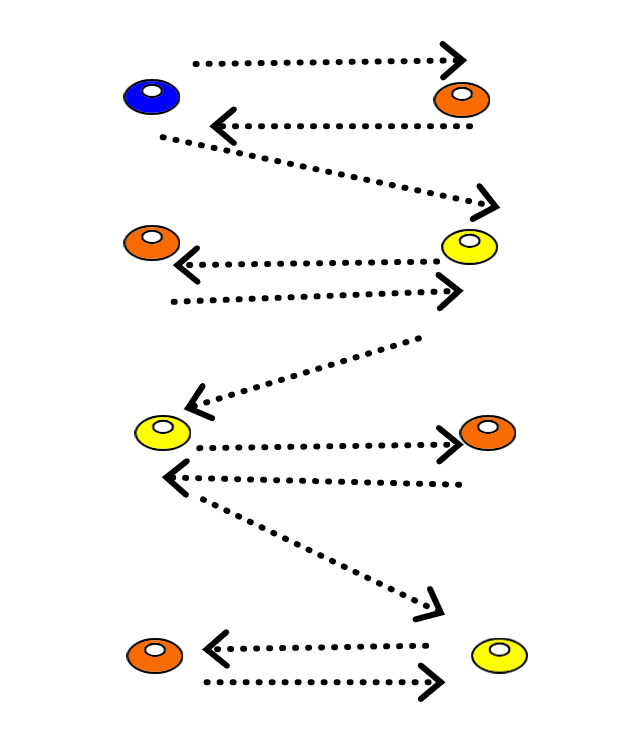
\includegraphics[width=.6\textwidth]{../img/Trimmed/lateral_shuddle}
    \end{minipage}
    \hspace{0.05\linewidth}
    \begin{minipage}{.6\linewidth} % Left column and width
        \textbf{Drill Description:}
        This agility drill works on lateral shuffling a critical skill for defenders. 
        \begin{enumerate}
            \setlength{\itemsep}{0pt}
            \setlength{\parskip}{0pt}
            \setlength{\parsep}{0pt}
            \item Players start at blue gate facing the line of 3 cones ahead of him,
            \item They shuttle side-ways to the orange cone, touch it with a finger then shuttle back to the blue cone touching it.
            \item Shuttle to diagonally to the yellow cone then to the orange cone, touching it, and back then to the yellow cone touching it, then shuttle diagonally to the next yellow cone.
            \item Keep repeating until the end.
        \end{enumerate}
    \end{minipage}
\end{minipage}
    %\vspace{12pt}
    %
    %\textbf{Coaching Points:}
    %\begin{itemize}
    %    \setlength{\itemsep}{0pt}
    %    \setlength{\parskip}{0pt}
    %    \setlength{\parsep}{0pt}
    %    \item TBD
    %\end{itemize}
\end{oddBlock}